\chapter{Etat de l'art}
\label{chap:analysis}

Ce chapitre dresse un état de l'art des avancées récentes dans la vision par ordinateur, la cartographie du potentiel solaire et l'analyse des toitures. Il examine les différentes méthodes et technologies développées dans ces domaines, en mettant l'accent sur les approches les plus innovantes et leurs applications pratiques.

\localtableofcontents

\newpage

% -----------------------------------------------------------------------------
\section{Introduction}
\par{L'évaluation du potentiel solaire des toitures est un élément clé de la transition énergétique urbaine. Sa précision dépend directement de la qualité et de la disponibilité des données utilisées, qui peuvent provenir de différentes sources avec des niveaux de détail variables.}

\par{Les méthodologies d'évaluation du potentiel solaire s'appuient principalement sur quatre types de données :}
\begin{enumerate}
    \item Données du cadastre
    \item Modèle tridimensionnel des bâtiments et du territoire
    \item Données géomatiques
    \item Orthophotos
\end{enumerate}

\par{La deuxième partie de ce chapitre va traiter de l'état de l'art en vision par ordinateur.}

% -----------------------------------------------------------------------------
\section{Évaluation du potentiel solaire des toitures}

% -----------------------------------------------------------------------------
\subsection{Analyse du potentiel photovoltaïque des toitures résidentielles en Andalousie}

\subsubsection{Contexte et objectifs}
\par{L'étude menée par \citeauthor{ordonez_analysis_2010} \cite{ordonez_analysis_2010} présente une analyse détaillée du potentiel de production d'énergie photovoltaïque sur les toitures résidentielles en Andalousie (Espagne). Cette région, avec une radiation solaire moyenne de 4,75 kWh/m² par jour et une superficie de 87 597 km², possède le plus fort potentiel solaire d'Europe.}

\subsubsection{Données}
\par{Les données utilisées dans cet article sont :}
\begin{itemize}
    \item Données du cadastre et les surfaces de toiture renseignées lors des autorisations de construire
    \item Orthophotos de google maps
\end{itemize}

\subsubsection{Méthodologie}
\par{La méthodologie repose sur trois volets complémentaires :}
\begin{itemize}
    \item L'analyse statistique des données du cadastre qui répartit les logements en trois types : les maisons individuelles ou jumelées, les maisons en bande, et les immeubles collectifs
    \item L'estimation des surfaces type de toit réellement utilisables pour les panneaux solaires, en prenant en compte tous les obstacles (cheminées, antennes, etc.), les zones d'ombre et les autres contraintes
    \item L'étude de l'ensoleillement moyen de la région et des performances des systèmes photovoltaïques, basée sur les caractéristiques techniques des panneaux disponibles
\end{itemize}

\subsubsection{Résultats principaux}
\par{L'analyse a permis d'identifier les potentiels suivants :}
\begin{itemize}
    \item La surface totale de toiture disponible est de 265,52 km², dont 218,52 km² (82,29\%) sont effectivement utilisables pour des installations photovoltaïques
    \item Le potentiel de production énergétique est estimé à 9,73 GWh/an pour des panneaux IS-170 et 9,38 GWh/an pour des panneaux IS-220
    \item Cette production permettrait de couvrir environ 78,89\% des besoins énergétiques du secteur résidentiel andalou, réduisant la dépendance énergétique extérieure à seulement 21,02\%
\end{itemize}

\subsubsection{Discussion et limites}
\par{Cette recherche démontre qu'il est possible d'estimer le potentiel solaire des toitures à partir de données déjà existantes, sans qu'il soit nécessaire d'investir dans l’acquisition de nouvelles données.}

\par{La méthodologie utilisée, bien que statistiquement solide, présente certaines limites. Notamment, elle s'appuie uniquement sur les données cadastrales issues des autorisations de construire et des enquêtes gouvernementales. Lors de la rédaction de cet article (2010), les auteurs se sont basés sur des données de 2000-2007. Actuellement, ils disposent de données \gls{lidar} \cite{nacional_plan_nodate} qui permettraient une évaluation plus précise et exhaustive du potentiel solaire pour l'Andalousie.}

% -----------------------------------------------------------------------------
\subsection{SolarNet}

\par{}

\subsubsection{Contexte et objectifs}

\subsubsection{Données}

\subsubsection{Méthodologie}

\subsubsection{Résultats principaux}

\subsubsection{Discussion et limites}

% -----------------------------------------------------------------------------
\subsection{Cadastre solaire}

\par{Il y a une multitude d'article dédiés à l'étude du potentiel solaire, la région de Genève est l'une des régions du monde avec le plus d'articles publiés après Wuhan (Chine) \cite{drozd_evaluating_2025}. \citeauthor{thebault_large-scale_2022} \cite{thebault_large-scale_2022} vont analyser la pertinence de la pose de panneaux solaire \acrshort{pv} au niveau du \gls{grandgeneve}}


\subsubsection{Contexte et objectifs}

\subsubsection{Données}

\subsubsection{Méthodologie}

\subsubsection{Résultats principaux}

\subsubsection{Discussion et limites}

% -----------------------------------------------------------------------------
\section{Vision par ordinateur}

% -----------------------------------------------------------------------------
\subsection{YOLO12}

% -----------------------------------------------------------------------------
\subsection{SolarNet}


\newpage
% -----------------------------------------------------------------------------

This chapter shows example of picture and also serves to populate the different lists: list of figures, list of tables, bibliography, and glossary.

\section{Tables}

This section contains an examples of table: \autoref{tab:esempio}

\begin{table}[h]
	\centering
	\begin{tabular}{ccc}
		\toprule
		name & weight & food \\ 
		\midrule
		mouse	& 10 g	& cheese \\
		cat	& 1 kg	& mice \\
		dog	& 10 kg	& cats \\
		t-rex	& 10 Mg	& dogs \\
		\bottomrule 
	\end{tabular}
	\caption[A floating table]{A floating table.}
	\label{tab:esempio}
\end{table}

\section{Figures}

This section contains examples of figures: \autoref{fig:galleria}, \autoref{fig:lorem}, \autoref{fig:ipsum}, \autoref{fig:dolor}, \autoref{fig:sit}

\begin{figure}[h] 
	\centering 
	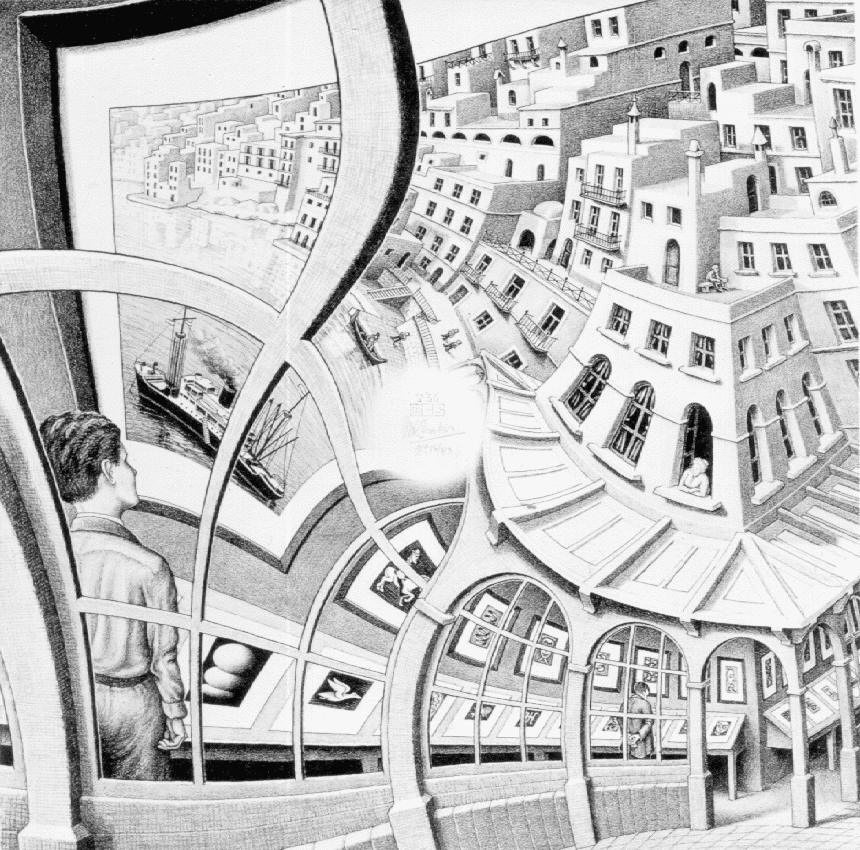
\includegraphics[width=0.5\columnwidth]{galleria_stampe} 
	\captionsource{A floating figure}{A floating figure: the lithograph \emph{Galleria di stampe}, of M.~Escher}{\url{http://www.mcescher.com/}}
	\label{fig:galleria} 
\end{figure}

\begin{figure}[h]
	\centering
	\begin{subfigure}[b]{0.45\textwidth}
		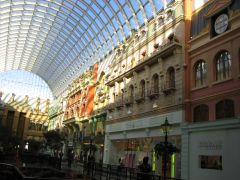
\includegraphics[width=\textwidth]{lorem}
		\caption{A gull}
		\label{fig:lorem}
	\end{subfigure}
	~ %add desired spacing between images, e. g. ~, \quad, \qquad, \hfill etc. 
	%(or a blank line to force the subfigure onto a new line)
	\begin{subfigure}[b]{0.45\textwidth}
		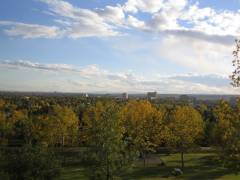
\includegraphics[width=\textwidth]{ipsum}
		\caption{A tiger}
		\label{fig:ipsum}
	\end{subfigure}
	~ %add desired spacing between images, e. g. ~, \quad, \qquad, \hfill etc. 
	%(or a blank line to force the subfigure onto a new line)
	\begin{subfigure}[b]{0.45\textwidth}
		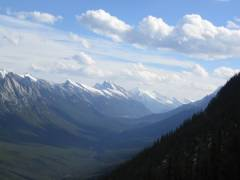
\includegraphics[width=\textwidth]{dolor}
		\caption{A mouse}
		\label{fig:dolor}
	\end{subfigure}
	~ %add desired spacing between images, e. g. ~, \quad, \qquad, \hfill etc. 
	%(or a blank line to force the subfigure onto a new line)
	\begin{subfigure}[b]{0.45\textwidth}
		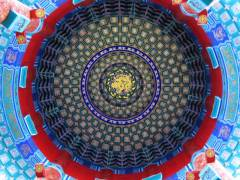
\includegraphics[width=\textwidth]{sit}
		\caption{A mouse}
		\label{fig:sit}
	\end{subfigure}
	\caption{Example subcaption}\label{fig:animals}
\end{figure}


% -----------------------------------------------------------------------------
\section{Code}

\autoref{lst:listing_example} shows an example of Java code rendered with minted.

\begin{listing}
	\javafile{02-main/listings/HelloWorld.java}
	\caption{Example of listing using the minted package}
	\label{lst:listing_example}
\end{listing}

% -----------------------------------------------------------------------------
\section{Other features}

Term (glossaries): \gls{latex}

Acronym (glossaries): \gls{api}

Citation (biblatex): \cite{paper_millwheel}

% -----------------------------------------------------------------------------
\section{Conclusion}

\blindtext
